\documentclass[11pt]{article}
\usepackage[utf8]{inputenc}
\usepackage[T1]{fontenc}
\usepackage{amsmath,amssymb,amsfonts}
\usepackage{tgtermes}
\usepackage{newtxmath}
\usepackage[version=4]{mhchem}
\usepackage{graphicx}
\usepackage{booktabs,longtable,tabularx,array}
\usepackage{siunitx}
\usepackage[margin=1in]{geometry}
\usepackage[hidelinks]{hyperref}
\usepackage{xr-hyper}
\externaldocument[main-]{main_R582}
\usepackage[numbers,sort&compress]{natbib}
\usepackage{xcolor}
\usepackage{authblk}
\usepackage{caption}
\usepackage[section]{placeins}
\usepackage{pdflscape}
\usepackage{tocloft}
\usepackage{microtype}

\captionsetup{font=small,labelfont=bf}
\setcounter{topnumber}{6}
\setcounter{totalnumber}{8}
\renewcommand{\topfraction}{0.95}
\renewcommand{\textfraction}{0.05}
\renewcommand{\floatpagefraction}{0.80}
\setlength{\floatsep}{8pt plus 2pt minus 2pt}
\setlength{\textfloatsep}{10pt plus 2pt minus 2pt}
\setlength{\cftsecnumwidth}{3.2em}
\setlength{\cftsubsecnumwidth}{4.4em}
\let\SIorigsubsection\subsection
\renewcommand{\subsection}{\FloatBarrier\SIorigsubsection}
\renewcommand{\thefigure}{S\arabic{figure}}
\renewcommand{\thetable}{S\arabic{table}}
\renewcommand{\theequation}{S\arabic{equation}}
\renewcommand{\thesection}{S\arabic{section}}
\renewcommand{\thesubsection}{\thesection.\arabic{subsection}}
\newcolumntype{Y}{>{\raggedright\arraybackslash}X}
\newcolumntype{C}[1]{>{\centering\arraybackslash}p{#1}}
\newcolumntype{P}[1]{>{\raggedright\arraybackslash}p{#1}}
\newcommand{\epss}{\varepsilon_{\mathrm{s}}}
\newcommand{\epsaux}{\varepsilon_{\mathrm{s,aux}}}
\newcommand{\iapp}{i_{\mathrm{app}}}
\newcommand{\csat}{c_{\mathrm{sat}}}
\newcommand{\Deff}{D_{\mathrm{eff}}}
\newcommand{\thetacal}{\theta_{\mathrm{cal}}}
\newcommand{\Rtheta}{R_{\theta}}
\newcommand{\Tpore}{T_{\mathrm{pore}}}
\newcommand{\thetaisland}{\theta_{\mathrm{island}}}
\newcommand{\mAhcm}{\si{mAh.cm^{-2}}}
\newcommand{\ci}{c_{\mathrm{I^-}}}
\newcommand{\cf}{c_{\mathrm{I_2}}^{\,\mathrm{free}}}
\DeclareSIUnit{\Molar}{M}
\graphicspath{{figures_R582/}}

\title{\bfseries Supplementary Information for\\[3pt]
\textit{A positive-electrode model separating iodine saturation from accessibility loss in zinc--iodine flow batteries}}
\author{\textit{[Verified author list and order required]}}
\affil{\textit{[Verified affiliations and corresponding-author details required]}}
\date{}

\begin{document}
\maketitle
\begingroup
\footnotesize
\setlength{\cftbeforesecskip}{1pt}
\setlength{\cftbeforesubsecskip}{0pt}
\tableofcontents
\endgroup
\clearpage

This Supplementary Information reports source identity, equations, numerical checks, complete field
inventories and bounded lower-scale calculations for the porous ZIFB positive electrode. Existing full-cell
records are descriptive anchors; molecular and mesoscale calculations are priors or comparators. Neither
evidence class identifies deposit morphology or independently validates an internal positive-electrode state.

Evidence classes are used consistently below. \texttt{E-EXP} denotes registered cell-level reanalysis;
\texttt{E-SIM}, a registered continuum solution or exported field; \texttt{E-CTRL}, a matched model-form
control; \texttt{E-COMP}, a deterministic lower-scale calculation; \texttt{E-POST}, a postprocessed scenario;
and \texttt{E-LIT/PRES}, a literature scale or prescribed input. These labels describe permitted inference,
not a ranking across unlike evidence types.

\section{Existing full-cell records and data provenance}

\subsection{Cell formats, source identity and inclusion rules}

Galvanostatic capacity, composition, compression and rate records were acquired in \SI{4}{cm^2} full cells
with a porous iodine positive electrode, zinc negative electrode and Nafion~212 separator. Separate cyclic-
voltammetry, chronoamperometry and impedance records used a \SI{1}{cm^2} three-electrode configuration with
an Ag/AgCl reference; no full-cell capacity is described as a three-electrode measurement. The physical
cell/file is the independent unit, and sequential cycles are repeated observations within that unit. The
retained acquisition records do not contain an independently logged experimental temperature. Continuum and
MD temperatures are therefore not assigned retrospectively to the experiments. Under correction ID
\texttt{EXP-META-001}, every legacy acquisition filename or condition field containing \texttt{NH4Cl},
including capitalization variants, denotes an experiment performed with NH4Br. Raw names, bytes and hashes
remain unchanged; derived labels use the corrected identity.

\begin{table}[!htbp]
\centering\footnotesize
\caption{\textbf{Experimental datasets, physical units and analysis roles.} Each row identifies the physical
cell or file unit, protocol role, processed source and permitted descriptive comparison. Dataset rows can
overlap in source cells and are not summed as an experiment-wide sample size.}
\label{tab:experimental-datasets}
\begin{tabularx}{\textwidth}{@{}P{2.25cm}P{1.45cm}P{1.55cm}P{1.6cm}YP{2.45cm}@{}}
\toprule
dataset & cell format & physical cells & cycles/files & processed source & evidence boundary\\
\midrule
late-charge derivative & \SI{4}{cm^2} full cell & 1 & 4 cycles &
\path{battery_experiment/02_processed_data/R581_G4_DVDQ_REBUILD} & within-cell estimator sensitivity only\\
composition series & \SI{4}{cm^2} full cell & 6 & 8 included run files; 315 classified cycles &
\path{battery_experiment/02_processed_data/R581_COMPOSITION_AXIS_REBUILD} & descriptive condition-associated envelopes; no population law\\
compression series & \SI{4}{cm^2} full cell & 4 & 108 of 110 reconstructed paired cycles retained &
\path{battery_experiment/02_processed_data/R581_COMPRESSION_EVIDENCE_REBUILD} & protocol brackets; one cell per thickness\\
pristine rate ladder & \SI{4}{cm^2} full cell & 1 & 29 cycles &
\path{battery_experiment/02_processed_data/R581_4M_RATE_HIGH_LOADING_REBUILD} & same-cell sequence at \SIrange{80}{360}{mA.cm^{-2}}\\
cross-protocol marker & \SI{4}{cm^2} full cell & 1 & 4 cycles & same processed directory & separate \SI{40}{mA.cm^{-2}} cell; not connected to the rate ladder\\
high-rate material proxy & \SI{4}{cm^2} full cell & 1 & 4 cycles & same processed directory & \SI{400}{mA.cm^{-2}} P350C-positive proxy; not a pristine continuation\\
electrochemical context & \SI{1}{cm^2} three-electrode cell & not pooled in R582 & separate CV/CA/EIS files &
\path{electrochemical} & method context only; not full-cell capacity evidence\\
\bottomrule
\end{tabularx}
\end{table}

\subsection{Sensitivity of the late-charge voltage feature}

The derivative analysis used the full-resolution pristine source, retained all four eligible sequential
cycles and interpolated voltage to a \SI{0.25}{mAh.cm^{-2}} grid. A cubic Savitzky--Golay derivative
\citep{Savitzky1964} with a
\SI{10.25}{mAh.cm^{-2}} physical window was the primary estimator; \SI{5.25}{mAh.cm^{-2}} and
\SI{15.25}{mAh.cm^{-2}} were prespecified sensitivity windows. Rise onset was the first point at
$Q\geq\SI{50}{mAh.cm^{-2}}$ exceeding the \SIrange{20}{50}{mAh.cm^{-2}} baseline median by four median
absolute deviations for five consecutive grid points. The derivative maximum was searched only from
\SI{50}{mAh.cm^{-2}} to $Q_{\mathrm{end}}-\SI{2.5}{mAh.cm^{-2}}$. These deterministic ranges are estimator
sensitivity, not confidence intervals. The derivative landmarks were not used to set $Q_s$ or
$Q_{\mathrm f,cal}$; $Q_{\mathrm f,cal}$ belongs to the pre-existing voltage-calibrated continuum branch.
The same full-cell trace is used separately in the reduced observation-layer fit in
Fig.~\ref{fig:si-voltage-degeneracy}, so this overlay is not independent validation.

\begin{figure}[!htbp]
\centering
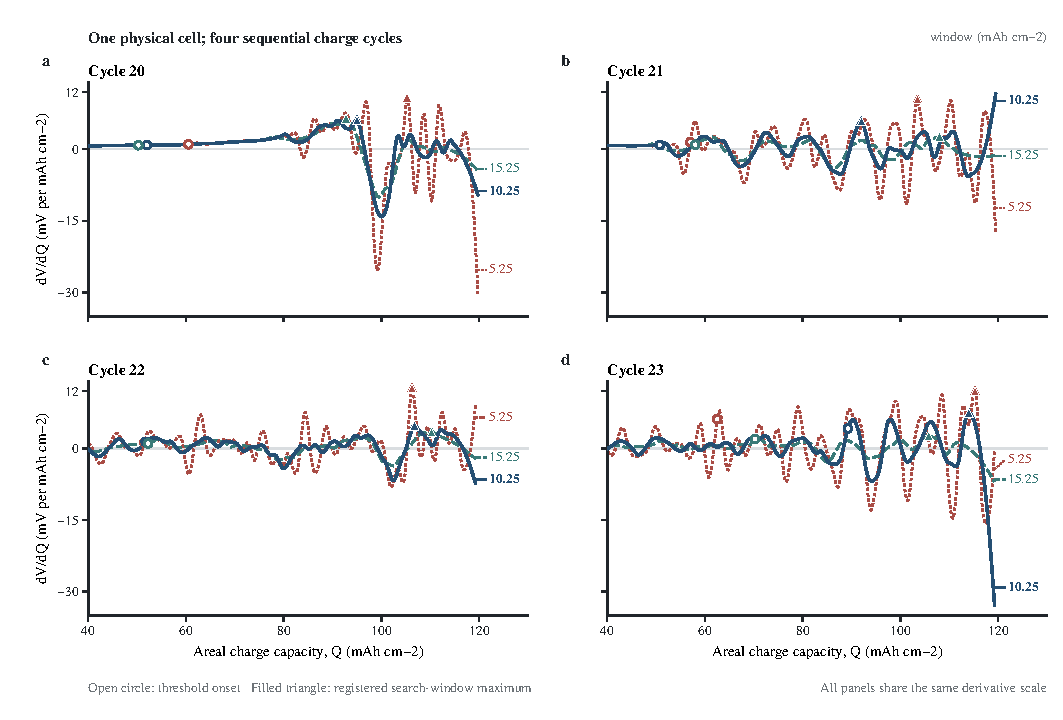
\includegraphics[width=\textwidth]{SIFig_R582_S1_derivative.pdf}
\caption{\textbf{Derivative-window sensitivity within one physical cell.} \textbf{a--d,} Full-cell charge-
curve derivatives for eligible cycles 20--23 of one pristine cell. Direct labels identify the three
prespecified physical windows; open circles mark registered rise onsets and filled triangles the registered
maxima. Boundary fluctuations outside the maximum-search interval remain visible. All panels share one
derivative scale. The cycles are within-cell repeated observations, not independent replicates. These
full-cell features do not identify a positive-electrode internal state. Derived electrolyte labels follow
\texttt{EXP-META-001}; raw records are unchanged.}
\label{fig:si-derivative}
\end{figure}

\begin{table}[!htbp]
\centering\small
\caption{\textbf{Voltage-rise onset and derivative maximum for every eligible cycle and smoothing window.}
The table reports deterministic estimator outputs for all cycle--window combinations rather than a selected
landmark. Capacities are in \si{mAh.cm^{-2}}.}
\label{tab:derivative-landmarks}
\begin{tabular}{cccc}
\toprule
cycle & window & rise onset & derivative maximum\\
\midrule
20 & 5.25 & 60.50 & 105.25\\
20 & 10.25 (primary) & 52.00 & 95.00\\
20 & 15.25 & 50.25 & 92.75\\
21 & 5.25 & 57.00 & 103.50\\
21 & 10.25 (primary) & 50.75 & 92.00\\
21 & 15.25 & 58.00 & 108.00\\
22 & 5.25 & 51.50 & 106.25\\
22 & 10.25 (primary) & 51.75 & 106.75\\
22 & 15.25 & 52.25 & 110.25\\
23 & 5.25 & 62.50 & 115.25\\
23 & 10.25 (primary) & 89.25 & 114.00\\
23 & 15.25 & 70.25 & 105.75\\
\bottomrule
\end{tabular}
\end{table}

Across the three windows, 11 of 12 rise onsets preceded the canonical modeled average-saturation marker,
whereas derivative maxima spanned \SIrange{92.0}{115.25}{mAh.cm^{-2}} and lay on both sides of the canonical
calibrated half-accessibility coordinate. The experimental feature is therefore distributed rather than a
single positive-electrode state validation.

\subsection{Descriptive supporting-electrolyte composition records}

The 0--4~M supporting-electrolyte series was acquired under an approximately \SI{80}{mA} total-current
program (\SIrange{19}{21}{mA.cm^{-2}} over \SI{4}{cm^2}). Six physical cells were conservatively identified
from 16 candidate paths and eight included run files. Continuations were stitched by acquisition identity and
time gap; duplicate snapshots were not counted as new cells. Cycles were first summarized within each cell.
No concentration law, optimum or population interval is fitted.

\begin{figure}[!htbp]
\centering
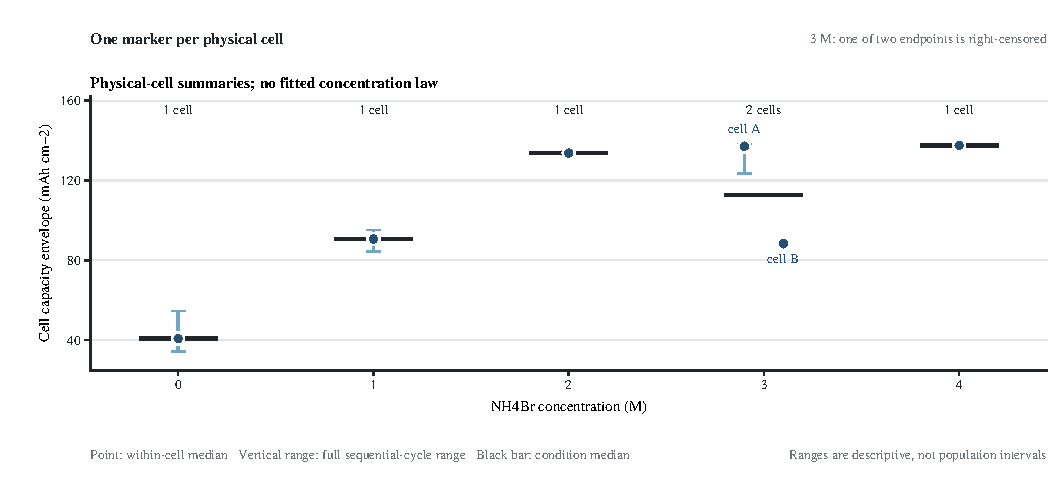
\includegraphics[width=\textwidth]{SIFig_R582_S2_composition.pdf}
\caption{\textbf{Cell-level descriptive capacity envelope across the existing composition records.} Each
filled marker is one physical cell and gives the maximum, across commanded levels, of the within-level median
delivered capacity. Vertical segments are full sequential-cycle ranges at the selected command, and short
black bars are condition medians. Physical-cell counts are 1/1/1/2/1 at 0/1/2/3/4~M NH4Br. The two
acquisitions at 2~M form one conservatively stitched cell; the two 3~M records are distinct, and one 3~M
endpoint is right-censored. The display is descriptive and does not identify an internal electrode state.}
\label{fig:si-composition}
\end{figure}

\begin{table}[!htbp]
\centering\small
\caption{\textbf{Cell-level composition summaries and CE-qualified command brackets.} The endpoint is the
maximum of the within-command median delivered capacity under the primary 85\% within-cell median-CE rule.
Observed last-pass/first-fail levels are command-resolution brackets, not confidence intervals.}
\label{tab:composition}
\begin{tabular}{cccl}
\toprule
NH4Br (M) & $n_{\mathrm{cell}}$ & capacity envelope (\mAhcm) & CE-qualified endpoint\\
\midrule
0 & 1 & 40.841 & $[40,60)$\\
1 & 1 & 90.667 & $[80,100)$\\
2 & 1 & 133.696 & $[140,160)$\\
3 & 2 & 137.096; 88.354 & $[140,160)$; $\geq100$ (right-censored)\\
4 & 1 & 137.539 & $[140,160)$\\
\bottomrule
\end{tabular}
\end{table}

\subsection{Descriptive compression records}

The 1.5, 2.5 and 3.0~mm records are explicit-thickness cells from the March 2025 campaign. The nominal 2.0~mm
point is an implicit-standard-thickness cell from a different acquisition batch and remains an open,
unconnected proxy. Each thickness represents one physical cell. The voltage-gap metric used in the source
reconstruction is the energy-weighted mean charge--discharge gap, not a mid-capacity difference.

\begin{figure}[!htbp]
\centering
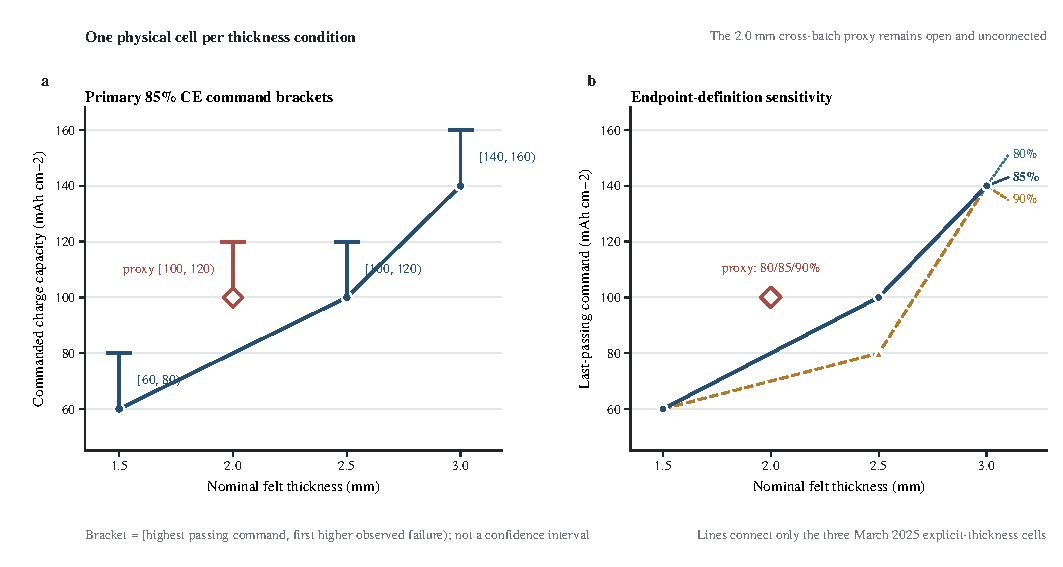
\includegraphics[width=\textwidth]{SIFig_R582_S3_compression.pdf}
\caption{\textbf{Protocol-bounded capacity brackets across existing felt-thickness cells.} \textbf{a,} Primary
85\% within-cell median-CE endpoint. The filled blue points connect only the three explicit March cells; the
open 2.0~mm cross-batch proxy is unconnected. \textbf{b,} Prespecified 80\%, 85\% and 90\% endpoint
sensitivity. Each bracket is program resolution, not a confidence interval. The data do not define a
population scaling law, pore-volume law or morphology relation.}
\label{fig:si-compression}
\end{figure}

\begin{table}[!htbp]
\centering\small
\caption{\textbf{Compression-series inclusion, endpoint brackets and delivered capacity.} Values use the
primary 85\% within-cell median-CE endpoint. Delivered capacity and CE are medians at the last passing level.}
\label{tab:compression}
\begin{tabular}{lcccccc}
\toprule
$L$ (mm) & role & $n_{\mathrm{cell}}$ & last pass & first fail & delivered (\mAhcm) & CE (\%)\\
\midrule
1.5 & explicit & 1 & 60 & 80 & 57.262 & 95.437\\
2.0 & cross-batch proxy & 1 & 100 & 120 & 95.271 & 95.271\\
2.5 & explicit & 1 & 100 & 120 & 85.956 & 85.956\\
3.0 & explicit & 1 & 140 & 160 & 135.511 & 96.793\\
\bottomrule
\end{tabular}
\end{table}

\subsection{Rate and high-loading records}

Only the \SIrange{80}{360}{mA.cm^{-2}} records form one same-cell pristine sequence. The
\SI{40}{mA.cm^{-2}} pristine source and \SI{400}{mA.cm^{-2}} P350C-positive proxy are independent cells and
remain unconnected. The pristine rate sequence is right-censored at \SI{360}{mA.cm^{-2}} with respect to a
95\% CE-failure current.

\begin{table}[!htbp]
\centering\small
\caption{\textbf{Source roles and efficiency summaries for the rate records.} Medians summarize sequential
cycles within one physical cell at each current. The 40 and \SI{400}{mA.cm^{-2}} sources do not extend the
pristine rate line.}
\label{tab:rate-records}
\begin{tabular}{llrrrr}
\toprule
source role & material identity & current (\si{mA.cm^{-2}}) & $n_{\mathrm{cell}}$ & $n_{\mathrm{cycle}}$ & median CE / EE (\%)\\
\midrule
cross-protocol marker & P-pristine/N-pristine & 40 & 1 & 4 & 94.911 / 86.754\\
rate-ladder start & P-pristine/N-pristine & 80 & 1 & 1 & 98.272 / 82.696\\
rate ladder & P-pristine/N-pristine & 120 & 1 & 4 & 98.368 / 76.317\\
rate ladder & P-pristine/N-pristine & 160 & 1 & 4 & 98.742 / 70.678\\
rate ladder & P-pristine/N-pristine & 200 & 1 & 4 & 98.776 / 65.533\\
rate ladder & P-pristine/N-pristine & 240 & 1 & 4 & 98.725 / 60.360\\
rate ladder & P-pristine/N-pristine & 280 & 1 & 4 & 97.770 / 55.217\\
rate ladder & P-pristine/N-pristine & 320 & 1 & 4 & 97.191 / 50.737\\
rate-ladder end & P-pristine/N-pristine & 360 & 1 & 4 & 96.703 / 47.163\\
material proxy only & P350C/N-pristine & 400 & 1 & 4 & 87.185 / 36.956\\
\bottomrule
\end{tabular}
\end{table}

These full-cell observations combine both electrodes, separator, shuttle and recovery losses. They can anchor
and stress-test a positive-electrode model but cannot validate free iodine, retained-solid inventory or
accessibility separately.

\section{Positive-electrode continuum formulation and computational identity}

\subsection{State variables and reaction balances}

The continuum calculation transports one lumped oxidized-iodine pool, $c_O$, rather than separate mobile
\ce{I3^-}, \ce{I2Br^-} and aqueous \ce{I2} fields. Remaining iodide is an algebraic stoichiometric inventory,
\begin{align}
c_R&=\max(c_{R,\mathrm{floor}},c_{R,0}-3c_O),\\
\varepsilon\,\partial_t c_O+\nabla\!\cdot(\mathbf{u}c_O-D_{O,\mathrm{eff}}\nabla c_O)
&=R_{\mathrm b}-R_{\mathrm{dep}}+(r_{\mathrm d}-r_{\mathrm p})/V_m .
\label{eq:species}
\end{align}
The local speciation buffer is
\begin{equation}
\beta=1+K_{\mathrm I}c_R+K_{\mathrm{Br}}c_{\mathrm{Br}},\qquad
\cf=c_O/\beta,\qquad S=\cf/\csat^{\mathrm{eff}},
\label{eq:speciation}
\end{equation}
with the implemented surface-effective stress also including the registered boundary-layer generation term.
Thus $c_R$, $\cf$ and $S$ are algebraic consequences of solved states and imposed closures, not additional
transported fields.

Charge is conserved through
\begin{equation}
i_v=a_{\mathrm b}j_{\mathrm b}+a_sj_{\mathrm{dep}},\qquad
\nabla\!\cdot\mathbf{i}_s=-i_v,\quad \nabla\!\cdot\mathbf{i}_l=i_v,
\quad \mathbf{i}_s=-\sigma_{s,\mathrm{eff}}\nabla\phi_s,
\quad \mathbf{i}_l=-\kappa_{l,\mathrm{eff}}\nabla\phi_l .
\label{eq:charge}
\end{equation}
The soluble path uses constant-exchange-current Butler--Volmer kinetics,
\begin{equation}
j_{\mathrm b}=i_0\!\left[\exp\!\left(\frac{\alpha_aF\eta}{RT}\right)-
\exp\!\left(-\frac{\alpha_cF\eta}{RT}\right)\right],\qquad
\eta=\phi_s-\phi_l-E_{\mathrm{eq}},
\label{eq:bv}
\end{equation}
where the implemented $E_{\mathrm{eq}}$ is an empirical total-pool Nernst-like relation, not a complete
activity model. A supersaturation-gated native deposited-solid path advances the retained-solid state,
\begin{align}
j_{\mathrm{dep}}&=i_{0,\mathrm{dep}}^{\mathrm{base}}\max(S_{\mathrm{local}}-1,0)
10^{\eta/A_a},\\
\partial_t\epss&=V_m\frac{a_sj_{\mathrm{dep}}}{2F}.
\label{eq:native-solid}
\end{align}
The distinct auxiliary states satisfy
\begin{align}
\partial_t\epsaux&=r_{\mathrm p}-r_{\mathrm d},\\
\partial_tN_{\mathrm{I_2}}&=\kappa_N(N_{\mathrm{target}}-N_{\mathrm{I_2}}),
\label{eq:auxiliary}
\end{align}
and are not substituted for $\epss$. The dimensionless $N_{\mathrm{I_2}}$ enters the calibrated relation
\begin{equation}
\thetacal=1-\exp\!\left[-6N_{\mathrm{I_2}}^{1/3}\varepsilon_{\mathrm{s,reg}}^{2/3}\right],
\qquad \Rtheta\equiv1-\thetacal .
\label{eq:rtheta}
\end{equation}
The native reaction-area identity contains a separate smooth pore factor,
\begin{equation}
\Tpore\equiv\left(\frac{K}{K_0}\right)^{1/2},\qquad
\frac{A_{\mathrm{bare}}}{A_0}=\Rtheta\Tpore,
\qquad a_{\mathrm b}=a_s\Rtheta\Tpore .
\label{eq:abare}
\end{equation}
Consequently, $1-\thetacal$ is $\Rtheta$, not the native $A_{\mathrm{bare}}/A_0$ field. The calibrated
half-accessibility coordinate $Q_{\mathrm f,cal}$ is defined by $\langle\thetacal\rangle=0.5$ (equivalently
$\langle\Rtheta\rangle=0.5$), not by halving the product in Eq.~\eqref{eq:abare}.

The remaining smooth feedback relations are
\begin{equation}
\varepsilon_{l,\mathrm{eff}}=\varepsilon-\epss,\qquad
\frac{K}{K_0}=\left(\frac{\varepsilon_{l,\mathrm{eff}}}{\varepsilon}\right)^3
\left(\frac{1-\varepsilon}{1-\varepsilon_{l,\mathrm{eff}}}\right)^2,\qquad
\{D,\kappa_l\}\propto\left(\frac{\varepsilon_{l,\mathrm{eff}}}{\varepsilon}\right)^{3/2}.
\label{eq:transport-closures}
\end{equation}

\begin{table}[!htbp]
\centering\footnotesize
\caption{\textbf{Model objects, equations, exported sources and evidence roles.} Primary solved states,
algebraic consequences, calibrated relations and prescribed inputs are distinguished explicitly.}
\label{tab:model-map}
\begin{tabularx}{\textwidth}{@{}P{2.25cm}P{2.55cm}P{2.15cm}P{1.25cm}Y@{}}
\toprule
object & source or equation & status & class & interpretation boundary\\
\midrule
$c_O$ & Eq.~\eqref{eq:species} & transported solved state & E-SIM & lumped oxidized pool; species-resolved transport is not solved\\
$c_R$ & Eq.~\eqref{eq:species}; \texttt{cI\_m\_surf\_avg} & algebraic consequence & E-SIM & reconstructed iodide inventory, not a second solved species\\
$\cf,S$ & Eq.~\eqref{eq:speciation}; \texttt{S\_surf} & algebraic consequence & E-SIM & modeled free-iodine stress; not a measured concentration field\\
$\epss$ & Eq.~\eqref{eq:native-solid}; \texttt{eps\_s\_pos} & native solved state & E-SIM & retained-solid fraction; not a deposit image\\
$\epsaux,N_{\mathrm{I_2}}$ & Eq.~\eqref{eq:auxiliary} & auxiliary ODE states & E-SIM & tracker and dimensionless dynamic state; neither replaces $\epss$\\
$\thetacal,\Rtheta$ & Eq.~\eqref{eq:rtheta}; \texttt{theta\_eff} & calibrated relation & E-SIM & calibration-controlled accessibility factor; not morphology or full native area\\
$\Tpore,A_{\mathrm{bare}}/A_0$ & Eq.~\eqref{eq:abare}; \texttt{A\_bare\_frac} & native algebraic closure & E-SIM & native area is $\Rtheta\Tpore$; $\Rtheta$ alone must not be relabelled as this field\\
porosity, $K/K_0$, $D$, $\kappa_l$ & Eq.~\eqref{eq:transport-closures} & smooth closures & E-SIM & mean-field transport channel; no local blockage is resolved\\
$\mathbf{u},p$ & \texttt{u\_native\_mag}, \texttt{p\_native} & solved hydraulic fields & E-SIM & $p$ is hydraulic pressure; no electrical-potential map is exported\\
$j_{\mathrm{total}}$ & Eq.~\eqref{eq:charge}; \texttt{j\_total} & solved reaction field & E-SIM & signed current is retained; non-positive nodes are not absolutized\\
terminal voltage & \texttt{voltage\_V} & galvanostatic output & E-SIM & conditional on the calibrated model and full-cell boundary representation\\
\bottomrule
\end{tabularx}
\end{table}

\subsection{Geometry, flow, reservoir, boundary and initial conditions}

The two-dimensional positive-electrode domain spans the compressed through-plane coordinate
$x\in[3,5]$~mm from current collector to separator and the flow-wise coordinate $y\in[0,20]$~mm. Mechanical
compression keeps felt-fibre inventory fixed,
\begin{equation}
(1-\varepsilon)L=\SI{0.30}{mm}.
\label{eq:compression-rule}
\end{equation}
Electrolyte flow obeys Darcy's relation
\begin{equation}
\mathbf{u}=-\frac{\kappa_0(K/K_0)}{\mu}\nabla p,
\qquad \nabla\!\cdot\mathbf{u}=0,
\label{eq:darcy}
\end{equation}
and is coupled to the electrochemical calculation through convection. The registered outlet reference is
$p_{\mathrm{out}}=0$; all displayed pressure is hydraulic pressure in pascals. Only the solved loading window
is interpreted. No mechanical-failure or deep extrapolation is assigned physical meaning.

A well-mixed reservoir of volume $V_{\mathrm{tank}}$ supplies the transported pool,
\begin{equation}
V_{\mathrm{tank}}\frac{\mathrm dc_O^{\mathrm{tank}}}{\mathrm dt}
=\dot V(c_O^{\mathrm{out}}-c_O^{\mathrm{tank}}).
\label{eq:tank}
\end{equation}
At the inlet, $c_O=c_O^{\mathrm{tank}}$ and the superficial flow is prescribed. The outlet has zero diffusive
species flux and $p=p_{\mathrm{out}}$. Iodine species have zero normal flux at collector and separator;
electronic current enters at the collector and ionic current leaves at the separator. Initial $c_O$ is uniform,
$c_R$ follows Eq.~\eqref{eq:species}, and $\epss=0$.

\subsection{Parameter roles}

\begin{table}[!htbp]
\centering\footnotesize
\caption{\textbf{Cell, geometry, protocol and electrochemical inputs.} Values are classified as recorded
hardware/protocol, prescribed scenario, calibrated relation or numerical model choice.}
\label{tab:cell-inputs}
\begin{tabularx}{\textwidth}{@{}P{3.25cm}P{2.0cm}P{3.35cm}Y@{}}
\toprule
quantity & symbol & value & role and provenance\\
\midrule
electrode area & $A$ & \SI{4}{cm^2} & recorded hardware\\
felt thickness; porosity rule & $L,\varepsilon(L)$ & \SI{2}{mm}; $1-\SI{0.30}{mm}/L$ & prescribed baseline and structural closure\\
specific area & $a_s$ & $4\times10^4~\si{m^{-1}}$ & empirical geometry scale; no independent area measurement\\
separator & --- & Nafion~212 ($\approx\SI{50}{\micro m}$) & recorded hardware\\
tank volume; flow & $V_{\mathrm{tank}},\dot V$ & \SI{25}{mL}; \SI{50}{mL.min^{-1}} & prescribed baseline protocol\\
temperature & $T$ & \SI{293.15}{K} & continuum-model setting; not assigned to experimental files\\
applied current density & $\iapp$ & \SI{400}{A.m^{-2}} (\SI{40}{mA.cm^{-2}}) & prescribed baseline\\
electrolyte condition & --- & \SI{1}{M} \ce{ZnI2} + \SI{4}{M} NH4Br & representative supporting-electrolyte condition\\
formal potential & $E^{0\prime}$ & \SI{0.548}{V} & prescribed reference; no present-electrolyte anchor\\
exchange current & $i_0$ & $5\times10^4~\si{A.m^{-2}}$ & fast-kinetics closure; not an intrinsic measurement\\
transfer coefficients & $\alpha_a,\alpha_c$ & $1,1$ & prescribed symmetric Butler--Volmer relation\\
liquid conductivity & $\kappa_l$ & \SI{20}{S.m^{-1}} & undocumented prescribed value; no raw conductivity record located\\
Nernst-like reference & $c_{\mathrm{ref}}$ & \SI{120}{mol.m^{-3}} & empirical total-pool reference\\
\bottomrule
\end{tabularx}
\end{table}

\begin{table}[!htbp]
\centering\footnotesize
\caption{\textbf{Transport, speciation and saturation inputs.} Transport and speciation values are lower-scale
or literature priors unless a present-electrolyte measurement record is identified.}
\label{tab:transport-inputs}
\begin{tabularx}{\textwidth}{@{}P{3.05cm}P{2.1cm}P{3.35cm}Y@{}}
\toprule
quantity & symbol & value & role and provenance\\
\midrule
free-\ce{I2} diffusivity & $D_{\ce{I2}}$ & $0.6\times10^{-9}~\si{m^2.s^{-1}}$ & lower-scale mobility prior; porous effective value remains model dependent\\
polyiodide diffusivity & $D_{\ce{I3^-}},D_{\ce{I2Br^-}}$ & $0.5\times10^{-9}~\si{m^2.s^{-1}}$ & force-field-limited lower-scale prior\\
mass-transfer length & $\delta$ & \SI{25}{\micro m} & prescribed sub-grid scenario; not measured\\
deposit-free permeability & $\kappa_0$ & $1.0\times10^{-10}~\si{m^2}$ & prescribed felt-scale value\\
viscosity; density & $\mu,\rho_l$ & $2.2\times10^{-3}~\si{Pa.s}$; \SI{1300}{kg.m^{-3}} & prescribed hydraulic values; not measured here\\
iodide complexation & $K_{\mathrm I}$ & $0.72~\si{m^3.mol^{-1}}$ & selected conditional prior near the $698\pm10~\si{M^{-1}}$ scale reported by Palmer \emph{et al.}\ \citep{Palmer1984}\\
bromide complexation & $K_{\mathrm{Br}}$ & $0.0115~\si{m^3.mol^{-1}}$ & rounded conditional prior near $12.2~\si{L.mol^{-1}}$ from Lee \emph{et al.}\ \citep{Lee2023}; system-specific formation precedent is not used as this number\\
intrinsic aqueous-\ce{I2} solubility & $\csat$ & \SI{1.33}{mol.m^{-3}} & dilute-water reference \citep{Ramette1965}\\
salting factor & $\gamma_{\mathrm{salt}}$ & 3; $\csat^{\mathrm{eff}}\approx\SI{0.44}{mol.m^{-3}}$ & bounded cross-salt prior, varied from 2 to 4 \citep{Palmer1984}\\
\ce{I2} molar volume & $V_m$ & $5.15\times10^{-5}~\si{m^3.mol^{-1}}$ & conversion from registered molar mass and density\\
\bottomrule
\end{tabularx}
\end{table}

\begin{table}[!htbp]
\centering\footnotesize
\caption{\textbf{Native-solid pathway, auxiliary-state constants and numerical regularizers.} The native solid
inventory and auxiliary dynamic states have distinct equations and evidential roles.}
\label{tab:solid-inputs}
\begin{tabularx}{\textwidth}{@{}P{3.4cm}P{2.35cm}P{2.6cm}Y@{}}
\toprule
quantity & symbol & value & role\\
\midrule
native-solid exchange scale & $i_{0,\mathrm{dep}}^{\mathrm{base}}$ & $0.05~\si{A.m^{-2}}$ & empirical deposited-species path\\
native-solid Tafel slope & $A_a$ & \SI{118}{mV} & prescribed path parameter\\
auxiliary formation/dissolution & $k_{\mathrm p},k_{\mathrm d}$ & $10^{-9},5\times10^{-9}~\si{m.s^{-1}}$ & empirical auxiliary-rate closures\\
dynamic-state relaxation & $\kappa_N$ & $10^{-2}~\si{s^{-1}}$ & calibrated relation\\
dynamic-state scales & $N_{\mathrm{ref}},N_{\mathrm{sup}},N_{\max}$ & $1,500,2\times10^7$ & dimensionless calibrated-state constants\\
overpotential scale & $\eta_{\mathrm{nuc}}$ & \SI{3}{mV} & calibrated dynamic-state parameter\\
supersaturation smoothing & --- & \SI{0.02}{mol.m^{-3}} & numerical smoothing\\
seed floor & $\nu_0$ & 0.03 & phenomenological initiation floor\\
solid-fraction regularizers & $\epss^{\mathrm{fl}},\epss^{\mathrm{sm}}$ & $10^{-9},10^{-8}$ & numerical regularizers\\
initial felt porosity & $\varepsilon_0$ & 0.85 & prescribed structural scenario\\
\bottomrule
\end{tabularx}
\end{table}

At the canonical endpoint, the native retained-solid fraction is $3.21926\times10^{-3}$ while the auxiliary
tracker is $1.08328\times10^{-6}$. The native path carries 0.5516\% of integrated charge and 27.994\% of the
endpoint positive current. These values demonstrate that the two states are not interchangeable.

\subsection{Computational identity and numerical provenance}

COMSOL Multiphysics 6.3.0.290 (COMSOL AB, Stockholm, Sweden) was used for the continuum calculations. The
baseline figures retain the registered R526 production identity, while the matched accessibility comparison
uses the convergence-qualified true-mesh pair.

\begin{table}[!htbp]
\centering\scriptsize
\caption{\textbf{Continuum-model identity, input hashes and numerical checks.} Original and archived solved
models were not modified. Matched calculations began from byte-identical copies.}
\label{tab:computational-identity}
\begin{tabularx}{\textwidth}{@{}P{2.5cm}P{3.6cm}YP{2.35cm}@{}}
\toprule
object & software object & immutable identity or setting & check\\
\midrule
canonical baseline & branch \texttt{PB-R526-J40-Q120-\allowbreak{}DSET5-v1} & study \texttt{stdR522}; solution \texttt{sol5}; dataset \texttt{dset5}; 1081 exported points over \texttt{range(0,10,10800)} & source of baseline fields and canonical event coordinates\\
source input copy & two independent copied \texttt{.mph} files & \texttt{4813B306F39330CC\allowbreak{}EAF819C4AB8815C5\allowbreak{}5A3DF8A04726741F\allowbreak{}33ACB801B8806B9B} & byte-identical before model-form change\\
fresh control & \texttt{stdR522/sol5/\allowbreak{}dsetR581Ctrl} & solved copy SHA-256 \texttt{B26D8FA00159C7EF\allowbreak{}90B5932886C54F28\allowbreak{}5BBBD8EBA899A0F7\allowbreak{}C62AAD7D8FBC6FED} & maximum voltage difference from historical trace: \SI{0.285}{mV}\\
physical-dense copy & \texttt{stdR522/sol5/\allowbreak{}dsetR581Phys} & only \texttt{cov\_theta\_surf} and \texttt{theta\_eff\_R520} changed to $1-\exp(-35.4\epss^{0.6222})$ & all parameter inventories byte-identical\\
tolerance pair & 1944 elements; $\mathrm{rtol}=3\times10^{-4}$ & separate control and physical copied solves & predeclared tolerance gate passed\\
true-mesh pair & 7776 elements; $\mathrm{rtol}=3\times10^{-4}$; minimum quality 0.198 & control timeseries SHA-256 \texttt{B6C0EAB603D17E94\allowbreak{}77CADAB04F6F0093\allowbreak{}D0C98261925561E5\allowbreak{}10C82B9203704569}; physical timeseries \texttt{22B8AE22303A850B\allowbreak{}AEA710E293992103\allowbreak{}C5783AB158B63F7E\allowbreak{}7ACD757561014AF8} & fourfold element-count gate passed\\
mesh response gate & true mesh versus same-tolerance 1944-element pair & $\Delta Q_s=0.0126$ (control), $0.1431~\mAhcm$ (physical); endpoint $\Delta V$ change \SI{0.0938}{mV} & all predeclared state and identity checks passed\\
\bottomrule
\end{tabularx}
\end{table}

\section{Extended positive-electrode state fields}

\subsection{Snapshot and event definitions}

Exact exports at $Q=0$, 80, 96, 100, 110 and \SI{120}{mAh.cm^{-2}} expose the progression before, between
and after the canonical averaged event coordinates. The $Q=100$ export is close to, but not identical with,
$Q_{\mathrm f,cal}=\SI{99.5901}{mAh.cm^{-2}}$. Local $S>1$ and native solid can occur before the electrode-
average $Q_s$ crossing.

\begin{table}[!htbp]
\centering\small
\caption{\textbf{Event definitions and exported snapshot roles.} Display capacities are exact exports;
$Q_s$ and $Q_{\mathrm f,cal}$ are interpolated electrode-average coordinates.}
\label{tab:snapshots}
\begin{tabularx}{\textwidth}{@{}P{2.3cm}P{3.0cm}Y@{}}
\toprule
coordinate (\mAhcm) & registered definition & display role\\
\midrule
$Q_s=83.0202$ & first upward crossing of $\langle S\rangle=1$ & canonical averaged saturation marker; not first local supersaturation\\
$Q_{\mathrm f,cal}=99.5901$ & $\langle\thetacal\rangle=0.5$, equivalently $\langle\Rtheta\rangle=0.5$ & calibrated accessibility coordinate; not $A_{\mathrm{bare}}/A_0=0.5$\\
0 & exact export & start of charge\\
80 & exact export & immediately before the average-saturation coordinate\\
96 & exact export & between $Q_s$ and $Q_{\mathrm f,cal}$\\
100 & exact export & nearest registered snapshot to $Q_{\mathrm f,cal}$\\
110 & exact export & post-half-accessibility progression\\
120 & exact export & canonical analysis endpoint\\
\bottomrule
\end{tabularx}
\end{table}

\subsection{State, function and reaction fields}

Figure~\ref{fig:si-state-fields} assembles the six registered positive-electrode exports using fixed row-wise
scales and nearest-neighbour rendering without image smoothing.

\begin{figure}[!htbp]
\centering
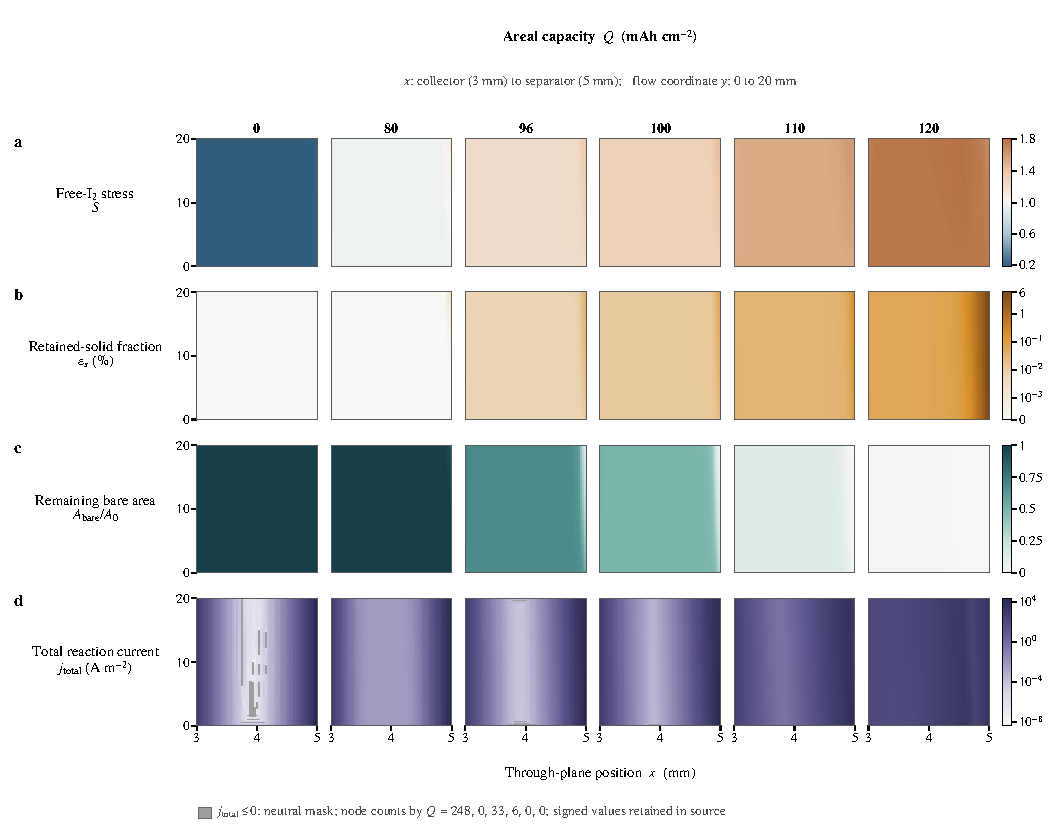
\includegraphics[width=\textwidth]{Fig_SI_R582_S4_state_function_fields.pdf}
\caption{\textbf{Six-capacity inventory of modeled positive-electrode state and reaction fields.} Columns show
$Q=0$, 80, 96, 100, 110 and \SI{120}{mAh.cm^{-2}}. \textbf{a,} Free-\ce{I2} stress $S$ on a shared scale
centred at $S=1$. \textbf{b,} Native retained-solid fraction $\epss$ on a shared symlogarithmic percentage
scale. \textbf{c,} Native remaining reaction-area fraction $A_{\mathrm{bare}}/A_0=\Rtheta\Tpore$ from the
registered \texttt{A\_bare\_frac} export. \textbf{d,} Total reaction-current density. Positive values use one
logarithmic scale; non-positive nodes are neutrally masked without taking absolute values. Their counts are
248, 0, 33, 6, 0 and 0 in column order, and signed values remain in the source table. Each map contains 5995
nodes and uses nearest-neighbour rendering without smoothing or clipping. These fields are model outputs, not
microscopy, deposit morphology, a blockage front or electrical potential.}
\label{fig:si-state-fields}
\end{figure}

\subsection{Hydraulic fields}

Figure~\ref{fig:si-hydraulic-fields} reports the corresponding smooth-permeability, velocity and hydraulic-
pressure exports on fixed row-wise scales.

\begin{figure}[!htbp]
\centering
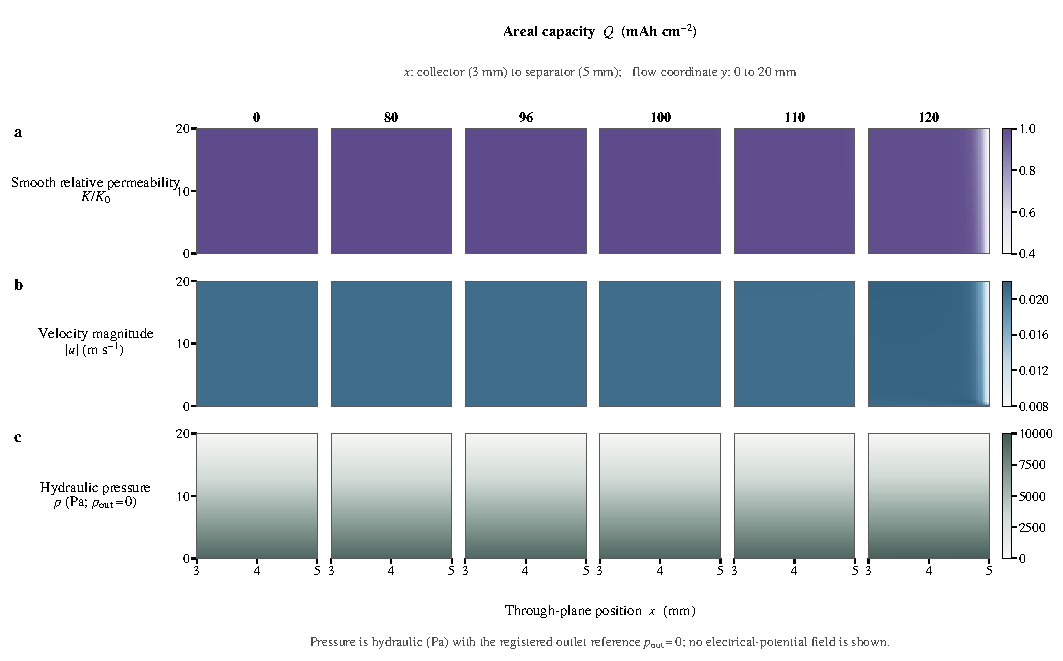
\includegraphics[width=\textwidth]{Fig_SI_R582_S5_hydraulic_fields.pdf}
\caption{\textbf{Hydraulic response across the same six positive-electrode states.} \textbf{a,} Smooth
relative permeability $K/K_0$. \textbf{b,} Native velocity magnitude in \si{m.s^{-1}}. \textbf{c,} Hydraulic
pressure in Pa relative to $p_{\mathrm{out}}=0$. Each row has one fixed scale across all capacities, and every
map contains the same 5995 exported nodes. The pressure field is hydraulic, not an electrical potential. The
smooth permeability channel does not resolve local pore closure or blockage.}
\label{fig:si-hydraulic-fields}
\end{figure}

\section{Accessibility-relation comparison, convergence and voltage identifiability}

\subsection{Matched model-form sensitivity}

The matched control and physical-dense calculations start from byte-identical copies. The control changes no
expression; the coupled physical-dense calculation changes only the two registered accessibility expressions
to the dense single-fibre comparator. A separate one-way shadow evaluates that comparator on the control
$\epss(Q)$ trajectory without feedback. These are three different objects.

\begin{table}[!htbp]
\centering\small
\caption{\textbf{Convergence-qualified matched accessibility comparison.} Changing only the accessibility
relation leaves the average saturation point nearly unchanged but alters later accessibility, solid inventory
and voltage. This is a controlled model-form sensitivity, not real-material causality or morphology
identification. Endpoint values are at \SI{120}{mAh.cm^{-2}}.}
\label{tab:matched-comparison}
\begin{tabularx}{\textwidth}{@{}P{3.8cm}YYY@{}}
\toprule
quantity & true-mesh control & one-way dense shadow & coupled physical dense\\
\midrule
$Q_s$ (\mAhcm) & 82.8903 & inherited control state & 82.8924\\
$Q(\thetacal=0.5)$ (\mAhcm) & 99.4637 & 118.6927 & not reached\\
endpoint $V$ (V) & 1.728364 & not a solve & 1.440208\\
endpoint $\epss$ & $3.15236\times10^{-3}$ & inherited control state & $6.58584\times10^{-4}$\\
endpoint $\theta$ & 0.989982 & 0.625898 & 0.309081\\
endpoint $\Rtheta=1-\theta$ & 0.0100178 & 0.374102 & 0.690919\\
endpoint $A_{\mathrm{bare}}/A_0$ & 0.00996125 & not evaluated as a native solve & 0.687120\\
endpoint $K/K_0$ & 0.957035 & inherited control state & 0.988976\\
\midrule
$V_{\mathrm{physical}}-V_{\mathrm{control}}$ & \multicolumn{3}{c}{$-288.156$~mV}\\
mesh-gate change in this difference & \multicolumn{3}{c}{0.0938~mV}\\
\bottomrule
\end{tabularx}
\end{table}

\subsection{Observation-layer identifiability}

The reduced observation layer fits a selected full-cell voltage interval with a baseline, linear capacity term
and one accessibility-related logarithmic contribution. It is an identifiability diagnostic, not a second
continuum solve. In this reduced layer, the varied accessibility coordinate is $\Rtheta$; it is not the native
$A_{\mathrm{bare}}/A_0=\Rtheta\Tpore$ field.

\begin{figure}[!htbp]
\centering
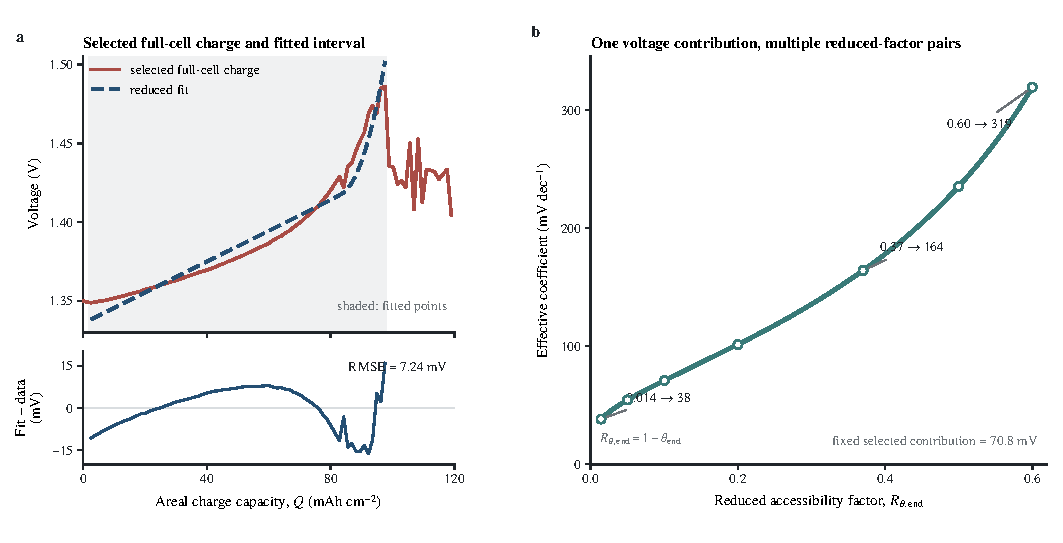
\includegraphics[width=\textwidth]{SIFig_R582_S6_voltage_degeneracy.pdf}
\caption{\textbf{Full-cell voltage fit and accessibility--coefficient degeneracy.} \textbf{a,} Selected
pristine full-cell charge trace and reduced observation-layer fit. The shaded interval contains 72 points from
2.672 to \SI{97.540}{mAh.cm^{-2}} in
$V=c_0+c_1Q+b_{\mathrm{eff}}\ln(1/\Rtheta)$; the lower axis shows fit minus data. The fit gives
$c_0=\SI{1.33554}{V}$, $c_1=9.819\times10^{-4}~\si{V.(mAh.cm^{-2})^{-1}}$,
$b_{\mathrm{eff}}=\SI{0.13622}{V}$ and RMSE \SI{7.24}{mV}. \textbf{b,} End-point $\Rtheta$--coefficient
pairs that preserve the selected \SI{70.813}{mV} accessibility-related voltage contribution. Open circles
are registered pairs and the line is the analytical relation. Here $\Rtheta$ is a reduced observation-layer
factor, not native remaining reaction area. Voltage therefore does not identify the inventory-to-accessibility
relation or deposit morphology uniquely.}
\label{fig:si-voltage-degeneracy}
\end{figure}

No internal-overpotential decomposition is used in the submission SI because it would add a conditional
mechanism separation not required by the R582 claims.

\section{Molecular bounds on placement and mobility}

\subsection{Periodic molecular-iodine calculations}

Periodic electronic-structure calculations used CP2K/Quickstep 2026.1
\citep{Kuhne2020CP2K,VandeVondele2005Quickstep}, PBE \citep{Perdew1996PBE}, D3(BJ)
\citep{Grimme2010D3,Grimme2011D3BJ}, DZVP-MOLOPT-SR-GTH basis sets
\citep{VandeVondele2007MOLOPT}, GTH pseudopotentials
\citep{Goedecker1996GTH,Hartwigsen1998GTH,Krack2005GTHPBE}, a 150~Ry density cutoff, a 30~Ry relative
cutoff and $\Gamma$-point sampling. Counterpoise-corrected single-point energies define the single-\ce{I2}
ordering \citep{Boys1970Counterpoise}. These finite-periodic-cell electronic energies are not solution free
energies, site populations or nucleation barriers.

\begin{table}[!htbp]
\centering\small
\caption{\textbf{Periodic single-\ce{I2} BSSE-corrected adsorption energies and two-\ce{I2}
compact-versus-separated electronic-energy diagnostic.} Single-\ce{I2} values are BSSE-corrected adsorption
energies within the declared calculations; two-\ce{I2} relative values compare the registered compact and
separated configurations. Both are used only as placement tendencies.}
\label{tab:dft-energies}
\begin{tabularx}{\textwidth}{@{}P{3.0cm}P{3.1cm}P{3.2cm}Y@{}}
\toprule
calculation & BSSE-corrected adsorption energy (eV) & relative reference (eV) & permitted use\\
\midrule
single \ce{I2}, C--OH & $-0.997724$ & $-0.595122$ versus basal & site-ordering prior\\
single \ce{I2}, C=O & $-0.848237$ & $-0.445635$ versus basal & site-ordering prior\\
single \ce{I2}, basal & $-0.402602$ & 0 & reference\\
single \ce{I2}, vacancy & $-0.318468$ & $+0.084134$ versus basal & site-ordering prior\\
compact two \ce{I2} at C--OH & --- & $-0.689291$ versus separated & configuration diagnostic\\
separated two-\ce{I2} reference & --- & 0 & reference\\
\bottomrule
\end{tabularx}
\end{table}

\begin{figure}[!htbp]
\centering
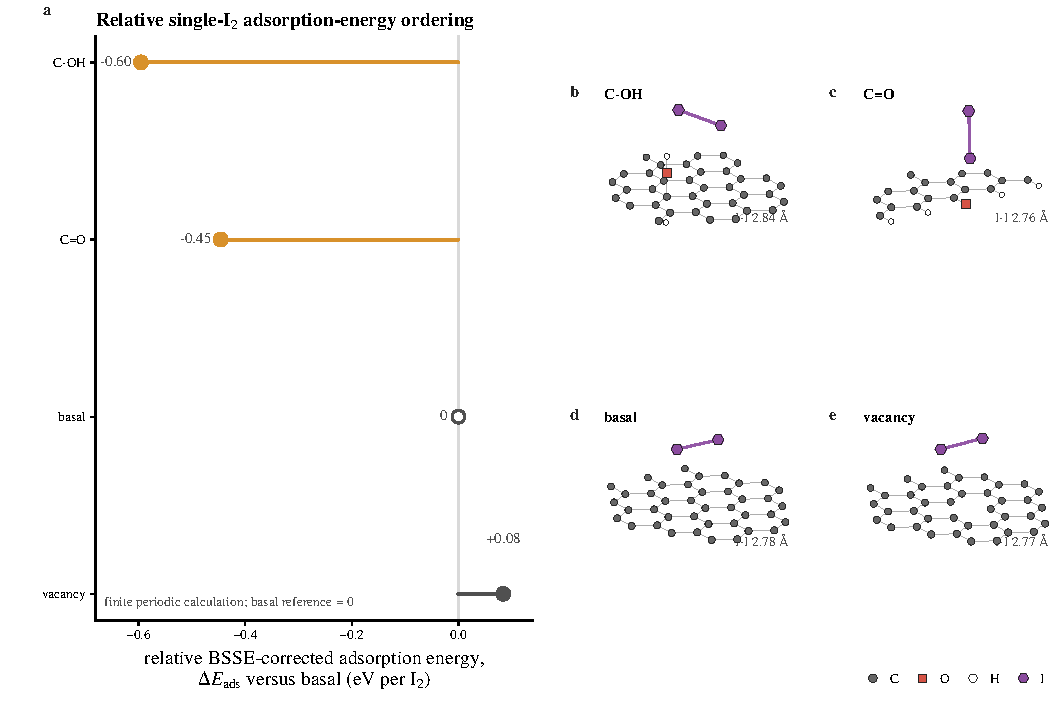
\includegraphics[width=\textwidth]{Fig_R582_SI07_single_I2_ordering.pdf}
\caption{\textbf{Relative single-\ce{I2} BSSE-corrected adsorption-energy ordering and optimized
geometries.} \textbf{a,} BSSE-corrected adsorption energies relative to the basal calculation.
\textbf{b--e,} Exact optimized
geometries in the same site order; displayed adjacency guides are distance based and do not assign bond order.
Within the declared finite periodic calculation, the tested C--OH and C=O motifs lie below basal carbon and
the vacancy lies slightly above it. The unavailable raw single-\ce{I2} charge-density fields are not used.}
\label{fig:si-single-i2}
\end{figure}

\begin{figure}[!ht]
\centering
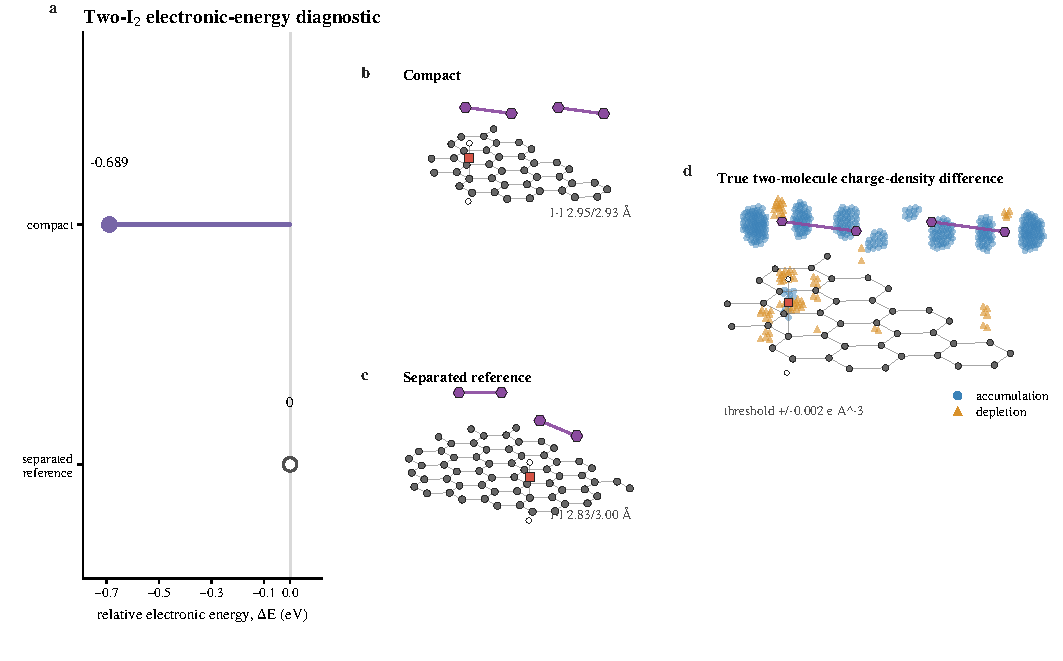
\includegraphics[width=\textwidth]{Fig_R582_SI08_two_I2_diagnostic.pdf}
\caption{\textbf{Compact and separated two-\ce{I2} configurations at the tested C--OH site.} \textbf{a,}
Registered compact-minus-separated electronic-energy comparison. \textbf{b,c,} Exact optimized compact and
separated geometries. \textbf{d,} Recoverable two-\ce{I2} charge-density-difference field, thresholded at
$\Delta\rho\geq+0.002$ or $\leq-0.002~e\,\text{\AA}^{-3}$ without smoothing or interpolation; 428
accumulation and 78 depletion points are retained. One periodic translation is used only to display the
compact cluster continuously. The compact configuration is \SI{0.689291}{eV} below the separated reference
within this calculation. The field is a diagnostic, not a reaction coordinate, solution equilibrium or
nucleation pathway.}
\label{fig:si-two-i2}
\end{figure}

\subsection{Molecular-dynamics carrier prior}

Classical MD used GROMACS 2026.0-conda\_forge \citep{Abraham2015GROMACS}, SPC/E water
\citep{Berendsen1987SPCE}, Joung--Cheatham-family halides \citep{Joung2008Ions}, Packmol initial
configurations \citep{Martinez2009Packmol}, and project-specific analogue parameters for the oxidized carriers.
Electronic-continuum charge scaling was compared with formal charges \citep{Leontyev2009ECC}. Five state-of-
charge compositions were run once under each charge parameterization. Four contiguous trajectory blocks
quantify within-trajectory stability and are not independent replicates.

\begin{table}[!htbp]
\centering\footnotesize
\caption{\textbf{MD protocol, estimator and force-field boundaries.} The protocol supplies a bounded carrier-
mobility prior; block statistics quantify within-trajectory stability only.}
\label{tab:md-protocol}
\begin{tabularx}{\textwidth}{@{}P{2.55cm}P{3.55cm}Y@{}}
\toprule
item & frozen implementation & evidence boundary\\
\midrule
software and cases & GROMACS 2026.0-conda\_forge; five SOC compositions at $q=0.8$ ECC and $q=1.0$ & one trajectory per composition and parameterization; ten cases are not replicates of one condition\\
trajectory & \SI{0.1}{ns} NVT, \SI{0.5}{ns} NPT, \SI{20}{ns} NVT production; \SI{2}{fs} step; \SI{5}{ps} frames & \SI{298.15}{K}; V-rescale thermostat \citep{Bussi2007VRescale}, C-rescale barostat in NPT \citep{Bernetti2020CRescale}, PME electrostatics \citep{Essmann1995PME}, \SI{1.0}{nm} real-space cutoffs\\
diffusion estimator & molecular-centre-of-mass Einstein MSD; lag fit \SIrange{2.51}{8.49}{ns} & four contiguous \SI{5}{ns} blocks provide a stability diagnostic, not replica SEM\\
base force fields & SPC/E water; Joung--Cheatham-style halides; SPC/E-compatible 12--6 \ce{Zn^2+}; compact \ce{NH4+}; neutral two-site \ce{I2} & several ion and molecular models are project approximations; no present-electrolyte force-field validation is claimed\\
polyhalides & GFN2-xTB/ALPB-water charge priors
\citep{Bannwarth2019GFN2xTB,Ehlert2021ALPB}; manual bonded and analogue Lennard--Jones terms & absolute
\ce{I3^-}/\ce{I2Br^-} diffusivities are high-uncertainty\\
viscosity & 18 planned Green--Kubo replica rows & required energy outputs are absent; these rows provide no result or uncertainty estimate\\
continuum use & bulk mobility ordering and range & porosity/tortuosity treatment is still required before use as $\Deff$\\
\bottomrule
\end{tabularx}
\end{table}

\begin{figure}[!htbp]
\centering
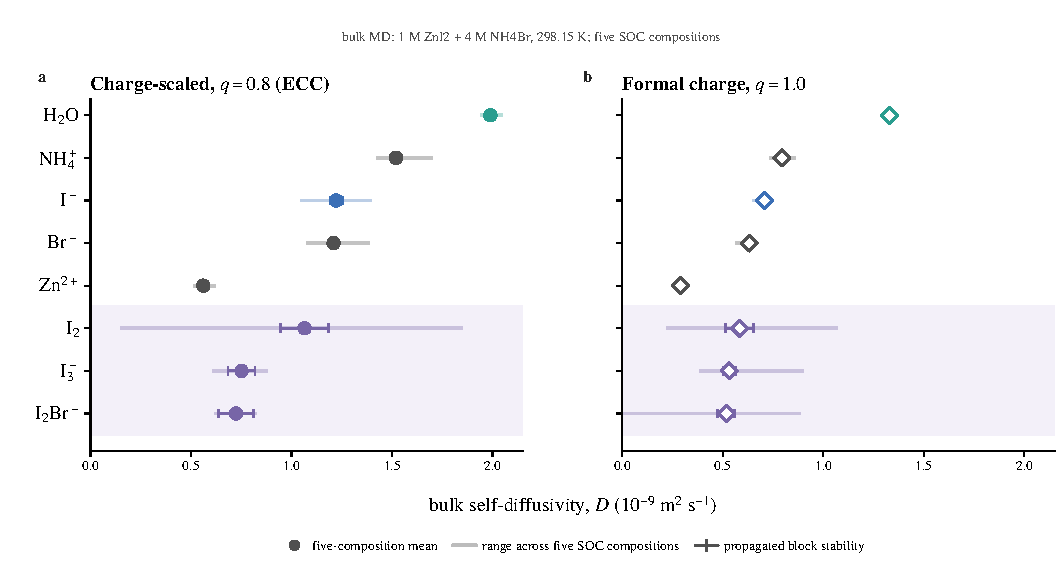
\includegraphics[width=\textwidth]{Fig_R582_SI09_md_carrier_ladder.pdf}
\caption{\textbf{Full carrier-mobility ladder under charge-scaled and formal-charge parameterizations.}
\textbf{a,} $q=0.8$ ECC. \textbf{b,} $q=1.0$ formal charges. The condition is 1~M \ce{ZnI2} + 4~M NH4Br
at \SI{298.15}{K}. Symbols are means across five different SOC compositions; thin spans show their min--max
range and capped bars the propagated four-block within-trajectory stability measure. Neither is replica
uncertainty. Oxidized-iodine carrier mobilities lie below iodide in both parameterizations, while absolute
values remain force-field dependent.}
\label{fig:si-md-ladder}
\end{figure}

\section{Single-fibre and pore-network comparator definitions}

\subsection{Idealized domains and boundary conditions}

Figure~\ref{fig:si-comparator-definitions} records the prescribed single-fibre and pore-network domains used
for the deterministic comparator calculations.

\begin{figure}[!htbp]
\centering
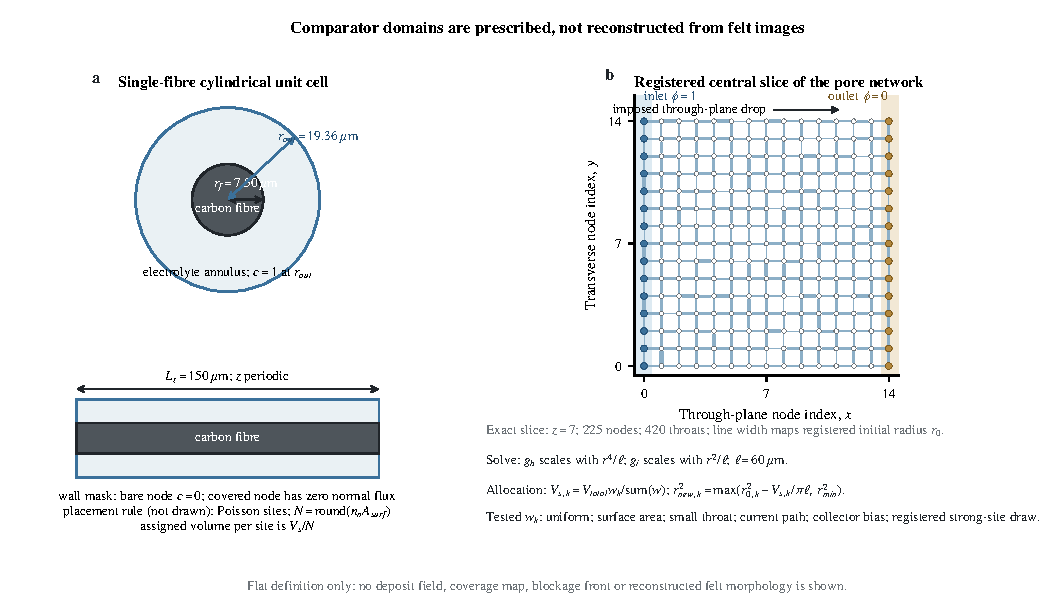
\includegraphics[width=\textwidth]{SIFig_R582_S10_comparator_definitions.pdf}
\caption{\textbf{Flat definitions of the single-fibre and pore-network comparator models.} \textbf{a,}
Orthographic views of the prescribed cylindrical unit cell
($r_f=\SI{7.50}{\micro m}$, $r_{\mathrm{out}}=\SI{19.36}{\micro m}$,
$L_z=\SI{150}{\micro m}$, $\varepsilon=0.85$). Normalized concentration is fixed at one at the outer radius;
a bare wall node has $c=0$, a covered node has zero normal flux, and azimuthal/axial directions are periodic.
\textbf{b,} Exact $z=7$ slice of the registered $15\times15\times15$ cubic network (225 nodes and 420 in-slice
throats). Line width maps initial throat radius; opposing faces have normalized Dirichlet values one and zero.
The \SI{60}{\micro m} lattice and displayed equations define conductance, allocation and radius update. These
are prescribed comparator domains, not images or reconstructions of the felt. No deposit field, solved
pressure, electrical potential, flux or blockage front is shown.}
\label{fig:si-comparator-definitions}
\end{figure}

\subsection{Accessibility families and threshold definitions}

The isolated-fibre calculations vary a prescribed placement density and precipitation fraction. Their
geometric $A/A_0$ is different from the continuum calibration coordinate $\Rtheta$. The latter can be plotted
only as a separately labelled comparator; it is not a native $A_{\mathrm{bare}}/A_0$ curve.

\begin{figure}[!htbp]
\centering
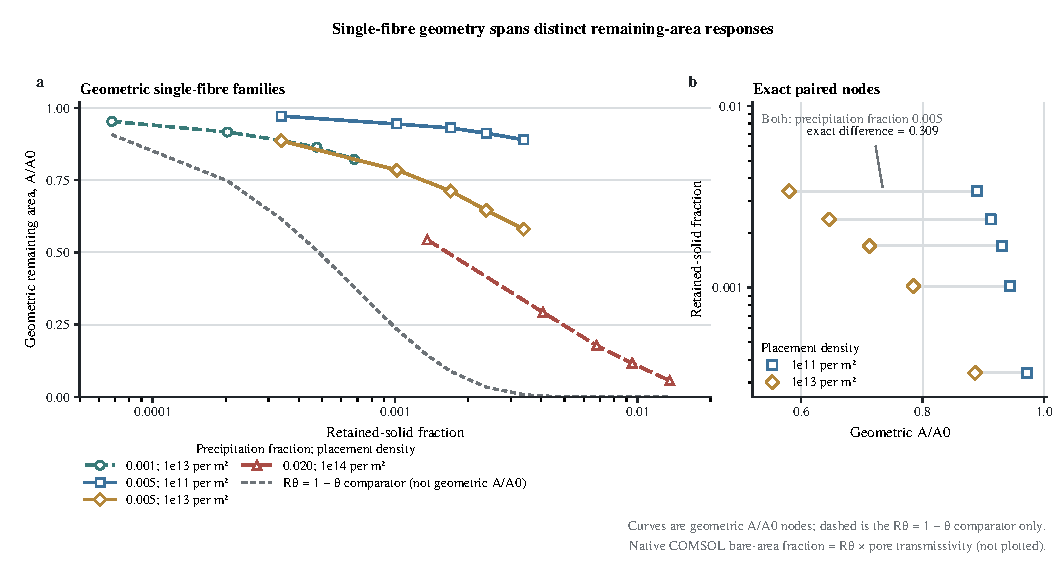
\includegraphics[width=\textwidth]{SIFig_R582_S11_accessibility_families.pdf}
\caption{\textbf{Remaining-accessibility families across the full tested placement-density range.}
\textbf{a,} Geometric single-fibre $A/A_0$ for all four registered comparator families. Lines connect five
computed nodes without fitting. The dashed grey curve is the separately calibrated continuum $\Rtheta$
relation sampled at the registered inventory nodes; it is not a geometric family and not native
$A_{\mathrm{bare}}/A_0$. \textbf{b,} Five shared inventory nodes for the two $\phi_{\mathrm{ppt}}=0.005$
families. Increasing prescribed placement density from $10^{11}$ to $10^{13}~\si{m^{-2}}$ changes geometric
remaining area by 0.085--0.309 over $\epss=3.39\times10^{-4}$ to $3.39\times10^{-3}$. These deterministic
comparators are not measured coverage, felt morphology or validation of the calibrated relation.}
\label{fig:si-accessibility-families}
\end{figure}

\begin{table}[!htbp]
\centering\small
\caption{\textbf{Definitions of calibrated, island-model and film-connectivity coordinates.} These quantities
have non-interchangeable definitions.}
\label{tab:thresholds}
\begin{tabularx}{\textwidth}{@{}P{3.0cm}P{2.5cm}P{3.2cm}Y@{}}
\toprule
coordinate & value in $\epss$ & definition & boundary\\
\midrule
calibrated trajectory readout & $1.18572\times10^{-4}$ & production trajectory when $\langle\thetacal\rangle=0.5$ & voltage-calibrated readout; not a material threshold and not $A_{\mathrm{bare}}/A_0=0.5$\\
dense-island half-area & $1.7973\times10^{-3}$ & $\thetaisland=0.5$ for $1-\exp(-35.4\epss^{0.6222})$ & idealized single-fibre comparator; direct discrete interpolation is approximately $1.91\times10^{-3}$\\
film-connectivity marker & $2.2324\times10^{-3}$ & registered geometric connected-film/percolation criterion & not a half-accessibility definition\\
\bottomrule
\end{tabularx}
\end{table}

\begin{landscape}
\section{Operating-variable scans and transport-channel controls}

\subsection{Complete scan matrix}

Each scan family changes one declared operating or model setting while holding its own remaining settings
fixed. Absolute endpoint voltages are not ranked across families with different fixed operating points.
$Q_s$ is obtained by linear interpolation across the first adjacent samples that bracket
$\langle S\rangle=1$; $Q_{\mathrm f,cal}$ is obtained analogously from $\langle\thetacal\rangle=0.5$. Endpoint
states in Table~\ref{tab:scan-matrix} report native $\epss$ and $\Rtheta=1-\thetacal$; full native reaction
area additionally contains $\Tpore$.

\scriptsize
\setlength{\tabcolsep}{3pt}
\begin{longtable}{@{}P{2.3cm}P{2.9cm}P{4.5cm}P{4.3cm}P{5.0cm}P{1.4cm}@{}}
\caption{\textbf{Tested operating/model-variable ranges and positive-electrode responses.} Lists follow
increasing setting. ``NR'' means the threshold was not reached within the stated solved trajectory. End states
are reported at \SI{120}{mAh.cm^{-2}} unless another endpoint is stated. The analytical row is postprocessed,
not a solved scan.}\label{tab:scan-matrix}\\
\toprule
family & tested settings & $Q_s$ (\mAhcm) & $Q_{\mathrm f,cal}$ (\mAhcm) & endpoint $\epss$; endpoint $\Rtheta$ & class\\
\midrule
\endfirsthead
\multicolumn{6}{l}{\tablename\ \thetable\ continued}\\
\toprule
family & tested settings & $Q_s$ (\mAhcm) & $Q_{\mathrm f,cal}$ (\mAhcm) & endpoint $\epss$; endpoint $\Rtheta$ & class\\
\midrule
\endhead
applied current & 20, 40 \si{mA.cm^{-2}} to $Q=120$; 80, 120 \si{mA.cm^{-2}} to $Q=40$ &
106.320; 83.020; $>40$; 8.391 & NR; 99.590; NR; 31.072 &
$1.402\times10^{-4}$; 0.52485 (20, $Q=120$). $3.219\times10^{-3}$; 0.01049 (40, $Q=120$).
$2.494\times10^{-7}$; 0.99881 (80, $Q=40$). $4.793\times10^{-4}$; 0.22052 (120, $Q=40$) & E-SIM\\
oxidized-carrier $\Deff/D_0$ & 0.5, 0.6, 0.8, 1.0, 1.2, 1.5, 2.0 &
45.034; 57.360; 73.131; 83.020; 89.972; 97.490; 106.205 &
61.099; 73.525; 89.503; 99.590; 106.748; 114.589; NR &
$\epss$: 0.166916; 0.108550; 0.032906; 0.003219; $4.657\times10^{-4}$; $2.178\times10^{-4}$; $7.324\times10^{-5}$.
$\Rtheta$: $3.14\times10^{-8}$; $2.4\times10^{-11}$; $2.063\times10^{-4}$; 0.01049; 0.07453; 0.28011; 0.66591 & E-SIM\\
linked felt geometry & 1.5, 2.0, 2.5, 3.0~mm; porosity changes with Eq.~\eqref{eq:compression-rule} &
82.385; 83.020; 83.657; 84.297 & 97.484; 99.590; 101.494; 103.253 &
$\epss$: 0.007188; 0.003219; 0.002065; $9.539\times10^{-4}$. $\Rtheta$: $1.967\times10^{-4}$; 0.01049; 0.02968; 0.07959 & E-SIM\\
solved flow & 25, 50, 100 \si{mL.min^{-1}} & 82.824; 83.020; 83.107 & 99.425; 99.590; 99.676 &
$\epss$: 0.004500; 0.003219; 0.002966. $\Rtheta$: 0.01062; 0.01049; 0.01049 & E-SIM\\
salting factor & $\gamma_{\mathrm{salt}}=2,3,4$ & 108.570; 83.020; 65.162 & NR; 99.590; 81.463 &
$\epss$: $5.651\times10^{-5}$; 0.003219; 0.064947. $\Rtheta$: 0.72363; 0.01049; $4.71\times10^{-8}$ & E-SIM / E-LIT-PRES\\
supporting-ligand concentration in the fixed model & 2, 3, 4, 5~M & 81.112; 82.066; 83.020; 83.973 &
97.496; 98.541; 99.590; 100.641 & $\epss$: 0.007474; 0.005626; 0.003219; 0.001897.
$\Rtheta$: 0.005015; 0.007343; 0.01049; 0.01505 & E-SIM\\
liquid conductivity & 10, 20, 40 \si{S.m^{-1}} & 83.028; 83.020; 83.013 & 99.600; 99.590; 99.581 &
$\epss$: 0.002996; 0.003219; 0.003353. $\Rtheta$: 0.01027; 0.01049; 0.01059 & E-SIM\\
solid conductivity & 80, 160, 320 \si{S.m^{-1}} & 83.015; 83.020; 83.026 & 99.589; 99.590; 99.592 &
$\epss$: 0.007193; 0.003219; 0.001598. $\Rtheta$: 0.01477; 0.01049; 0.008226 & E-SIM\\
wetted/specific-area factor & $0.5,1.0$; no registered converged $2\times$ trajectory & 83.017; 83.020 & 103.316; 99.590 &
$\epss$: $5.102\times10^{-4}$; 0.003219. $\Rtheta$: 0.05678; 0.01049 & E-SIM\\
analytical boundary-layer flow & 25, 50, 100 \si{mL.min^{-1}}, $m=0.5$ & 74.992; 83.022; 88.733 & not evaluated &
no solved endpoint state; only the generation contribution is rescaled & E-POST\\
smooth-permeability substitution & endpoint at $Q=120~\mAhcm$ & no registered $Q_s$ response & not evaluated &
network-minus-baseline endpoint voltage $+1.271$~mV; $K/K_0=0.98250$ versus 0.95629 & E-SIM\\
\bottomrule
\end{longtable}
\end{landscape}

Among the selected operating and transport variables carried into main Fig.~\ref{main-fig:operating-levers},
applied current and oxidized-carrier diffusivity produce the largest resolved movements in $Q_s$. The
prescribed $\gamma_{\mathrm{salt}}=2$--4 sensitivity spans a larger total response, but it is an
E-LIT/PRES prior rather than a fitted electrolyte law or independent experimental axis. The linked felt and
solved-flow families move the marker much less. Conductivity primarily changes the voltage/current-
distribution channel, while the saturation marker remains effectively fixed.

\subsection{Analytical sub-grid flow scenario}

\begin{figure}[!htbp]
\centering
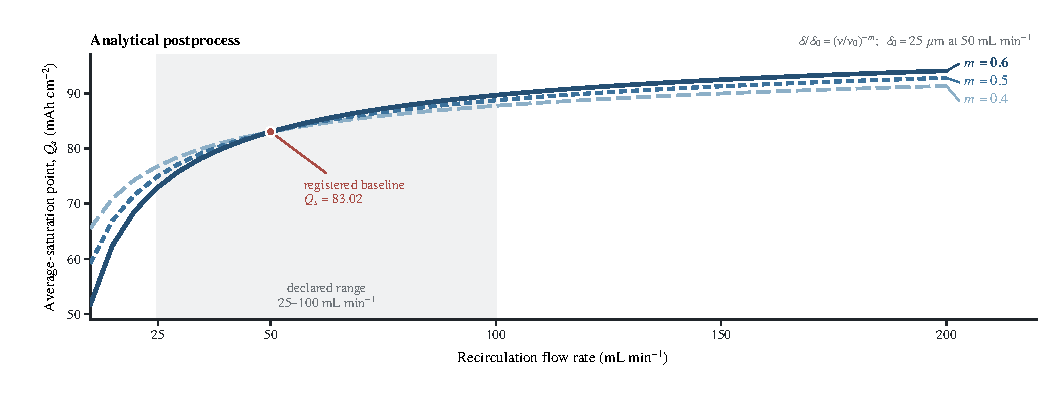
\includegraphics[width=\textwidth]{SIFig_R582_S12_flow_postprocess.pdf}
\caption{\textbf{Conditional flow dependence of the analytical boundary-layer scenario.} The registered
baseline was postprocessed with $\delta/\delta_0=(v/v_0)^{-m}$ for $m=0.4$, 0.5 and 0.6, with
$\delta_0=\SI{25}{\micro m}$ at \SI{50}{mL.min^{-1}}. All curves pass through
$Q_s=\SI{83.020}{mAh.cm^{-2}}$ at nominal flow. The shaded band marks \SIrange{25}{100}{mL.min^{-1}}; the
$m=0.5$ scenario moves $Q_s$ from 74.992 to \SI{88.733}{mAh.cm^{-2}}. These are registered analytical
evaluations that rescale only sub-grid generation stress, not a full flow-dependent boundary-layer solve or a
measured mass-transfer law.}
\label{fig:si-flow-postprocess}
\end{figure}

\subsection{Smooth-permeability substitution}

Figure~\ref{fig:si-permeability} compares the matched smooth-permeability paths and their voltage difference;
the calculation does not resolve local pore-throat blockage.

\begin{figure}[!htbp]
\centering
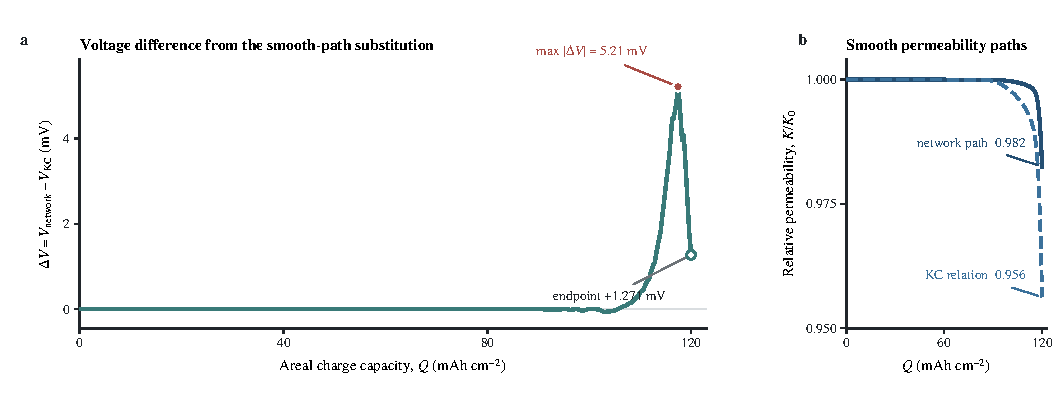
\includegraphics[width=\textwidth]{SIFig_R582_S13_smooth_permeability.pdf}
\caption{\textbf{Voltage response to replacing the smooth permeability relation.} \textbf{a,} Voltage
difference between the re-solve using the pore-network-derived smooth path and the matched Kozeny--Carman
baseline. The maximum absolute difference is \SI{5.214}{mV} at \SI{117.444}{mAh.cm^{-2}}; the difference at
\SI{120}{mAh.cm^{-2}} is $+\SI{1.271}{mV}$. \textbf{b,} Corresponding smooth $K/K_0$ paths; endpoint values
are 0.98250 and 0.95629. This control addresses smooth bulk permeability only. Local pore-throat blockage is
not resolved or excluded.}
\label{fig:si-permeability}
\end{figure}

\subsection{Transport-channel accounting}

\begin{table}[!htbp]
\centering\footnotesize
\caption{\textbf{Transport channels represented, approximated and excluded.} Accessibility, diffusive transfer
and smooth hydraulic permeability are distinct model channels; local pore blockage is not resolved.}
\label{tab:transport-channels}
\begin{tabularx}{\textwidth}{@{}P{2.55cm}P{2.7cm}P{2.2cm}Y@{}}
\toprule
channel & variable or relation & representation & permitted conclusion\\
\midrule
calibration-controlled accessibility & $\Rtheta=1-\thetacal$ & algebraic calibrated relation & changes the kinetic area factor; $Q_{\mathrm f,cal}$ is defined by $\thetacal=0.5$\\
native reaction area & $A_{\mathrm{bare}}/A_0=\Rtheta\Tpore$ & product of calibrated and smooth-pore factors & native area export is not identical to $\Rtheta$\\
diffusive transfer & $\Deff,\delta$ & solved effective diffusion plus prescribed sub-grid length & controls generation stress; absolute values remain prior dependent\\
smooth hydraulics & $K(\epss),\mu,\mathbf{u},p$ & Darcy flow with smooth permeability & supports in-window smooth pressure/velocity response only\\
charge transport & $\sigma_s,\kappa_l$ & solved current-conservation channel & can redistribute current and voltage without moving the saturation marker appreciably\\
lumped speciation & $c_O,c_R,\beta$ & one transported oxidized pool plus algebraic partition & no species-resolved polyiodide field or equilibrium validation\\
local blockage & pore-throat closure, shells, fronts & excluded & no claim about discrete blockage, pore closure or deposit morphology\\
\bottomrule
\end{tabularx}
\end{table}

\section{Scope, evidence boundaries and reproducibility}

\subsection{Consolidated claim boundaries}

\begin{table}[!htbp]
\centering\scriptsize
\caption{\textbf{Scope and bounds of the positive-electrode analysis.} Each row links a data or modeling limit
to the maximum supported claim.}
\label{tab:bounds}
\begin{tabularx}{\textwidth}{@{}P{2.7cm}P{2.0cm}YP{3.4cm}@{}}
\toprule
topic & class & direct support & maximum claim\\
\midrule
full-cell voltage identifiability & E-EXP/E-POST & reduced voltage fit and coefficient trade-off & voltage does not uniquely identify the inventory-to-accessibility relation\\
accessibility relation & E-SIM/E-CTRL & calibrated $\Rtheta$ and one matched alternative & model-form sensitivity, not true deposit morphology\\
native reaction area identity & E-SIM & exported $A_{\mathrm{bare}}/A_0=\Rtheta\Tpore$ & $\Rtheta$ alone is not the native area field\\
threshold definitions & E-SIM/E-COMP & calibrated, island-half and film-connectivity coordinates & definitions are non-interchangeable; none is a measured material threshold\\
prescribed/literature constants & E-LIT/PRES & documented input values and sensitivity scans & conditional parameter dependence, not present-electrolyte property identification\\
representative supporting electrolyte & E-EXP/E-LIT/PRES & corrected records and fixed model condition & an experimental/model boundary condition, not the central mechanism or a transferable electrolyte law\\
sparse experiments & E-EXP & one cell per condition except two at 3~M; one cell per thickness & descriptive within-cell records only; no population optimum or universal law\\
smooth versus local hydraulics & E-SIM & Darcy field and smooth-permeability control & small smooth in-window penalty does not exclude local blockage\\
lumped oxidized carrier & E-SIM & one transported $c_O$ state & no separate \ce{I3^-}, \ce{I2Br^-} or aqueous-\ce{I2} transport claim\\
electrode-resolved validation & E-EXP & full-cell voltage/capacity anchors & no independent validation of free iodine, retained solid or accessibility\\
molecular calculations & E-COMP & finite-cell energies and force-field MD & placement/mobility bounds only; no solution equilibrium or nucleation kinetics\\
comparator geometry & E-COMP & prescribed fibre and network calculations & not imaging or reconstruction of the felt\\
unexported fields & --- & registered spatial table lacks electrical potentials & no electrical-potential map or inference\\
outside solved domain & --- & negative electrode, shuttle, discharge reset and membrane damage not solved & no mechanistic conclusion for these processes\\
\bottomrule
\end{tabularx}
\end{table}

\subsection{Data and code identity}

The \href{https://github.com/ccyyyYyzz/ZIFB000/tree/r582-zifb-positive-electrode-reproducibility-v1/R582_PUBLICATION_REPRODUCIBILITY}{immutable tagged R582 reproducibility release} contains
plotted source tables and deterministic renderers for all 19 main and supplementary figures,
the exact manuscript and Supplementary Information sources, registered continuum-model input hashes and
study/solution/dataset identities, the adopted single-$\ce{I2}$ CP2K input/output identities, and exact
topology, parameter, protocol, metadata and log identities for the ten reported GROMACS cases. The
operator-confirmed \texttt{EXP-META-001} manifest records that every affected legacy \texttt{NH4Cl}/
\texttt{NH4CL} label denotes \ce{NH4Br} while preserving raw filenames and hashes. Raw acquisition files,
molecular trajectories and original solved \texttt{.mph} files are not duplicated in the lightweight
repository; their availability boundary and registered identities are documented there. New continuum
calculations operate only on copied, separately named and hash-registered models. No repository DOI had
been assigned at submission.

Negative-electrode morphology, shuttle, discharge reset and membrane damage lie outside the solved domain.
No negative-electrode calculation is displayed. The submission SI also excludes an internal-overpotential
decomposition, unrebuildable single-\ce{I2} charge-density artwork, hypothetical electrolyte extrapolation and
far-beyond-window mechanical or hydraulic-failure narratives.

\bibliographystyle{unsrtnat}
\bibliography{refs}

\end{document}
